\subsection{Exrahieren von Gestenkandidaten}
\label{sec:gesture_extraction}
Die Lichtsensorenmatrix liefert einen kontinuierlichen Strom an Bildern. Dabei limitiert die Verarbeitungszeit eines Bildes die Anzahl an Bilder pro Sekunde. Als Gestenkandidat wird eine Folge von Bildern definiert, die
ein Ereignis einschließt. In diesem Fall wird das Ereignis durch die Veränderung im gleitenden Mittelwert der Helligkeit definiert, d. h. sobald der gleitende Mittelwert unterschritten wird ein Gestenkandidat
angefangen aufgenommen zu werden und sobald die Lichtverhältnisse zu dem Wert zurückkehren wird die Aufnahme beendet. Der gleitende Mittelwert wird dabei immer angepasst, wenn kein Gestenkandidat aufgenommen wird, um
sich den veränderden Lichtverhältnissen anzupassen. Da leichte Veränderungen natürlich sind, muss eine Toleranzgrenze von 10\% unterschritten werden, damit die Aufnahme gestartet wird. Dies hat als Folge, dass der Anfang
und das Ende nicht vollständig sind. Aus diesem Grund schlug Kubik zusätzlich vor am Anfang und Ende weitere Bilder anzufügen \cite{kubikThesis}.
\begin{figure}
    \usetikzlibrary{arrows,automata,positioning}
    \centering
    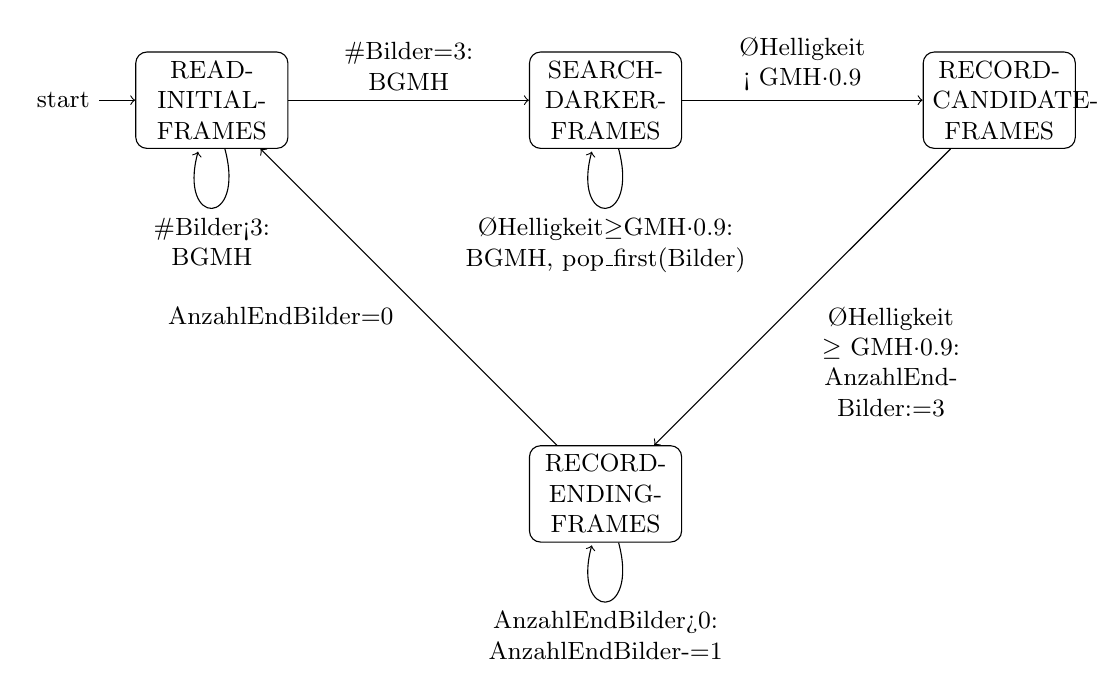
\begin{tikzpicture}[
        block/.style={
        draw,
        fill=white,
        text width=0.14*\columnwidth,
        anchor=west,
        minimum height=1cm,
        rounded corners
        },
        font=\small,
        on grid, auto,
        node distance=5cm
    ]
        \node [block,align=center,initial] (s0) {READ-INITIAL-FRAMES};
        \node [block,align=center] (s1) [right of=s0] {SEARCH-DARKER-FRAMES};
        \node [block,align=center] (s2) [right of=s1] {RECORD-CANDIDATE-FRAMES};
        \node [block,align=center] (s3) [below of=s1] {RECORD-ENDING-FRAMES};
        \path [->, text width=2cm, align=center] (s0) edge [loop below] node {\#Bilder<3: BGMH} (s0);
        \path [->, text width=2cm, align=center] (s0) edge node {\#Bilder=3: BGMH} (s1);
        \path [->, text width=4cm, align=center] (s1) edge [loop below] node {ØHelligkeit$\geq$GMH$\cdot 0.9$: BGMH, pop\_first(Bilder)} (s1);
        \path [->, text width=3cm, align=center] (s1) edge node {ØHelligkeit < GMH$\cdot 0.9$} (s2);
        \path [->, text width=2cm, align=center] (s2) edge node {ØHelligkeit $\geq$ GMH$\cdot 0.9$: AnzahlEndBilder:=3} (s3);
        \path [->, text width=3cm, align=center] (s3) edge [loop below] node {AnzahlEndBilder>0: AnzahlEndBilder-=1} (s3);
        \path [->, text width=3cm, align=center] (s3) edge node {AnzahlEndBilder=0} (s0);
    \end{tikzpicture}
    \caption{Implementierung von Kubik's Algorithmus um Gestenkandidaten zu erkennen von Dr. Marcus Venzke. BGMH steht für die Aktion \glqq \textbf{B}erechnung \textbf{G}leitender \textbf{M}ittelwert der \textbf{H}elligkeit\grqq und GMH steht für die Variable \glqq \textbf{G}leitender \textbf{M}ittelwert der \textbf{H}elligkeit\grqq.}
    \label{fig:venzkeAlgoImpl}
\end{figure}
\newline
\newline
Abbildung \ref{fig:venzkeAlgoImpl} zeigt die konkrete Implementierung dieses Algorithmus mit einem Zustandsautomaten, der von Dr. Marcus Venzke entwickelt wurde. In jedem Zustand wird das aktuelle Bild dem Puffer angefügt.
Der Automat verbleibt im Zustand \texttt{READ-INITIAL-FRAMES} bis der Puffer 3 Bilder enthält und passt stets den gleitenden Mittelwert der Helligkeit an. Anschließend geht der Automat in den Zustand
\texttt{SEARCH-DARKER-FRAMES} über, indem er weiterhin den gleitenden Mittelwert anpasst und immer das erste Bild aus dem Puffer entfernt, da lediglich 3 Bilder jeweils vor dem Aufnehmen und nach dem Aufnehmen des
Gestenkandidates angefügt werden sollen. Sobald die Durchschnittshelligkeit 90\% des gleitenden Mittelwerts unterschreitet wird die Aufnahme begonnen. Der Automat geht in den Zustand \texttt{RECORD-CANDIDATE-FRAMES}
über. Dort verbleibt der Automat solange bis die Durchschnittshelligkeit 90\% des gleitenden Mittelwerts überschreitet, woraufhin der Automat in den Zustand \texttt{RECORD-ENDING-FRAMES} über geht, indem die letzten 3
Bilder an den Puffer angehängt werden. Sobald 3 Bilder angehängt wurden, wird der Puffer dem Klassifizierer übergeben und anschließend der Zustandsautomat zurückgesetzt, woraufhin der Automat in den initialen
Zustand wieder übergeht.